\documentclass[a4paper,11pt]{jreport}


%本文中で図を貼りつけるためのパッケージを定義する。
\usepackage{amsmath}
\usepackage{stmaryrd}
\usepackage{amsfonts}
\usepackage{amssymb}
\usepackage{theorem}
\usepackage[dvipdfmx]{graphicx}
\usepackage{moreverb}
\usepackage{ascmac}
\usepackage{caption}
\usepackage{comment}
\usepackage{here}

%本文の書式を定義する。
\setlength{\topmargin}{0cm}
\setlength{\oddsidemargin}{1cm}
\setlength{\evensidemargin}{-1cm}
\setlength{\topmargin}{0cm}
\setlength{\textwidth}{14cm}
\setlength{\textheight}{21cm}
\setlength{\headheight}{2cm}

\renewcommand{\baselinestretch}{1.2}

\pagestyle{headings}

%%%%%%    TEXT START %%%%
\begin{document}
\pagenumbering{roman}
\setcounter{page}{0}

%%%%%   TITLE PAGE  %%%%%

%============================================================%
%      title.tex		表紙
%============================================================%

\begin{titlepage}
{\Large 平成31年度修士論文}\\

\setlength{\baselineskip}{13mm}
\parbox{\hsize}{
\vspace*{10mm}
\hspace*{\fill}
{\Large お茶の水女子大学大学院 博士前期課程
\vspace*{3mm}
\hspace*{\fill}\\\hspace*{\fill}
人間文化創成科学研究科 理学専攻 情報科学コース\hspace*{\fill}}}\\
\vspace*{8mm}

\begin{center}
  \textbf{
    \huge \textbf{Blocklyをベースにした\\OCamlビジュアルプログラミングエディタ}}
  \vspace*{20mm}
  
  \begin{figure}[h]
    \begin{center}
      \scalebox{1.2}{
\includegraphics{ocha_logo}}
    \end{center}
  \end{figure}
  \vspace*{20mm}
  
  {\LARGE
    \begin{tabular}{@{}lcl@{\quad}l}
      著者氏名 & : & 松本 晴香(学籍番号 1740664)\\[-1mm] \hline
      指導教官 & : & 理学部 情報科学科 准教授  & 浅井 健一\\[-1mm] \hline
    \end{tabular}
  }\\
  \vspace*{18mm}
  {\LARGE 平成 31 年 3 月}
\end{center}

\end{titlepage}


\newpage
\setcounter{page}{0}
\chapter*{要旨}


{\bf キーワード:}\ 

\newpage
\setcounter{page}{0}
\chapter*{Abstract}

We present OCaml Blockly, OCaml visual programming editor based on Blockly.
Blockly is a JavaScript library for creating visual block programming languages.
Blockly makes it impossible to cause a syntax error since constructed set of blocks always represents an abstract syntax tree.
However, Blockly does not deal with semantic errors, so it allows users to create a program which does not compile.

OCaml Blockly provides UI which prevents users from constructing blocks with any compile errors.
Blocks in OCaml Blockly change their colors and shapes using their data types inferred by its Hindley–Milner type system.
OCaml Blockly visually represents information of variables such as their types, bindings, and scopes.
Additionally, we support bidirectional converters between OCaml code and blocks in OCaml Blockly.
It helps beginners get used to text-based coding.
We show the design and implementation of OCaml Blockly and discuss future tasks toward practical uses.

{\bf Keywords:}\ Visual programming editor, OCaml, JavaScript, Blockly



%%%%%   CONTENTS %%%%%
\tableofcontents

%\listoffigures

\chapter{序論}\label{chap:intro}

関数型言語の初学者が関数型言語を学び始めたとき,
数々の本質的でない問題に陥りやすい.
変数に何らかの値を再代入しようとしてシンタックスエラーを起こしたり,
Int型とFloat型を持つ値を足し合わせようとして型エラーになってしまうことがある.
関数型言語のシンタックスや静的型付けに慣れていない初学者にとって,
テキストエディタは入力の自由度が高すぎるため,
エラーの原因を特定するのはしばしば困難である.

プログラミング初学者がプログラミング学習のために用いるツールの1つにビジュアルプログラミング環境がある\cite{Viscuit,Scratch,Snap}.
ビジュアルプログラミング環境では,テキストではなく,視覚的なオブジェクトを組み合わせることでプログラミングを行う.
例えば,近松らの\cite{HaskellVP}は,
変数や構文をノードで表し,ノードを線で繋いで値の入出力の関係を制御することによって,
Haskellプログラムをグラフとして表現する.

一方で,Googleの提供するBlockly \cite{Blockly}はブラウザにおけるビジュアルプログラミング環境構築のライブラリとして配布されているオープンソースプロジェクトであり,完全にクライアントサイドのみで動く.
ブロックの描画や移動,組み立てなどといったユーザインタフェースに関わる実装はライブラリ側が全て行なっているため,
ブロックに表示する文字や入出力の関係を定義するだけで,カスタマイズされたブロックを持つビジュアルプログラミング環境を作ることができる.
実装言語はJavaScriptであり,ブロックの描画にはSVGやCSSが活用されている.
また,Blocklyの標準のブロックであれば,ユーザが組み立てたブロック群から,JavaScript,Pythonなどといったスクリプト言語に変換することができる.

% グラフ型のビジュアルプログラミング言語との比較.なぜブロック型を採用したか.見た目的に取っつきやすい.Blocklyは開発者向けなので改造しやすい.
% 構文木とブロックが一対一対応であるのが視覚的にわかりやすく,シンタックスエラーが起こり得ない.
% ブロック型は関数型言語の上で重要な入出力の関係を載せるのに向いていない\cite{HaskellVP}が,(なにか主張を書く)
% なぜOCamlなのか
% sytaxになれる
本研究では,既に洗練されたユーザインタフェースが用意されていることや,構文木と一対一対応をしていて,テキストを連想しやすいことから,
BlocklyをベースとしてOCamlビジュアルプログラミング環境を実装し,これをOCaml Blocklyと名付けた.
OCaml Blocklyでは,不正なプログラムを表すブロックを組み立てることをユーザインタフェースによって制限する.
また,各ブロックが持つ型を形や色で表して,視覚的に出力する.%のように
関数型言語の初学者が,OCaml Blocklyの元でOCamlプログラミングを行うことで,以下の利点を得られることを期待している.
\begin{itemize}
  \item OCamlのシンタックスに慣れる.
  \item 自身が組み立てようとするプログラムが不正なものであることに瞬時に気づくことができ,テキストベースよりもストレスが少なく,OCamlプログラミングの本質を優先的に学習できる.
  \item 静的型付けを理解する.%OCamlのセマンティックスになれる
\end{itemize}
%関数型言語初学者がOCamlを学習する際の導入段階に使用し,シームレスにテキストベースによるプログラミングに繋がるようにすることが狙いである.
また,ブロックによるプログラミングによってOCamlの言語仕様に慣れ親しんだのち,シームレスにテキストベースによるプログラミングに繋がるように,本研究ではブロックとOCamlコードの相互変換の実装を行った.

本論文の構成を以下に示す.まず,{\bf 第\ref{chap:blocklyWord}章}でBlockly固有の用語を説明し,
{\bf 第\ref{chap:senko}章}にて関連研究とその問題点について分析し,その問題点を踏まえて本研究が将来的に達成すべき目標と,
本論文で達成するべき目標を示す.
次に,{\bf 第\ref{chap:features}章}で本論文が実装した主な機能を紹介し,
その各機能の実装の詳細を{\bf 第\ref{chap:impl}章}にて説明する.
{\bf 第\ref{chap:converter}章}でブロックとOCamlコードとの相互変換を行うためのシステムの構成を述べる.
{\bf 第\ref{chap:todo}章}で本システムの現状をまとめ,最終的な目標の達成のために実現されるべき課題を整理し,考察する.
最後に,{\bf 第\ref{chap:conclusion}章}にて本論文をまとめ,今後のさらなる展望について言及する.

\pagenumbering{arabic}

\chapter{関連研究}

自分が目的とした研究課題の動向や理論・手法などについて関連する先行研究に
ついて説明する.

\chapter{関連研究と目標}\label{chap:senko}

%この節では,Blocklyを関数型言語に拡張した2つの関連研究について述べる.
Blocklyに型付けを行った関連研究に,
Lernerらによる{\it Polymorphic Blocks} \cite{Typed-Blockly}がある.
ターゲット言語はOCamlではなく,擬似的な言語を対象にしている.
Int型やBool型といったプリミティブな型ごとにブロックのコネクタの部分の形を変え,Function型やList型といったパラメタ付き型についても再帰的に型の形を描画し,型変数については各コネクタを固有の色でハイライトすることにより,型変数を含めた型をわかりやすく視覚的に捉えられるようになっている(図\ref{fig:polyBlockList}).
型の視覚化を実現するために用いられているテクニックについて説明する.
まず,ブロックの入出力を表す各コネクタに型表現を添付する.Int型ならば,出力コネクタにIntの型表現が加えられ,List型ならば,各入力コネクタに任意の型変数表現 $\alpha$ が,出力コネクタにはその型変数 $\alpha$ をパラメタとして持つList型表現が保存される.型変数にはそれぞれランダムに生成した色を持たせておく.ある2つのコネクタがお互いに接続するときには,それぞれのコネクタについた型表現の単一化を行う.あとはブロックの描画時に,コネクタに添付された型が指す表現ごとに別の形や色を描画すればよい.これにより,ユーザの動作に基づいて動的に変わる型をブロックの上に描画することを実現している.

しかし,\cite{Typed-Blockly}では,不正なプログラムの組み立てを許してしまう(図\ref{fig:unboundValue}).
また,一度単一化された型はブロックを外しても元に戻らないことや,変数宣言の構文,let多相\cite{AkaHon}をサポートしていないなど,本研究が求める関数型言語初学者向けのツールとして活用するためには不完全な部分が多く見受けられる.

\begin{figure}[t]
 \centering
 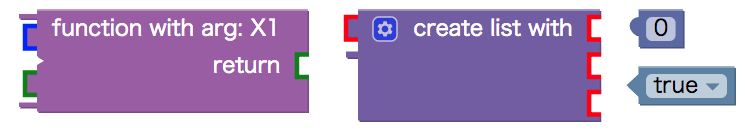
\includegraphics[scale=0.4]{img/blockEx.png}
 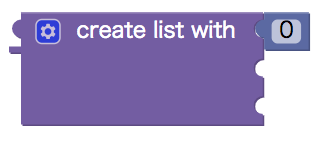
\includegraphics[scale=0.4]{img/intList.png} % TODO:余白合わせて!
 \caption{{\it Polymorphic Blocks}でのブロックの例.始めList型のパラメタの型は決定していないため,型変数を意味するハイライトが赤色で示されているが(右上),Int 型のブロックを接続させると,ハイライトが消え Int 型の形に変更される(下).\label{fig:polyBlockList}}
 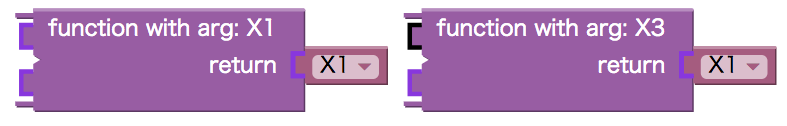
\includegraphics[scale=0.4]{img/unboundValue.png}
 \caption{{\it Polymorphic Blocks}で組み立てた2つのラムダ式ブロック.左のブロックはラムダ式として正当だが,右のブロックでは入れ子になったブロックが表す変数X1が未定義なってしまう.\label{fig:unboundValue}}
\end{figure}

他の関連研究としては,FunBlocks \cite{FunBlocks}がある.
これはCodeWorld \cite{CodeWorld} というHaskellプログラミングの学習環境をBlockly上に実現したものである.
\cite{Typed-Blockly}と同様に型や型変数を視覚的に描画する方法を取っているが,
let多相やブロックを外したときの型の単一化の解除を行うなど,型システムは\cite{Typed-Blockly}よりも拡張されている.
一方で,スコープという概念がないために図\ref{fig:unboundValue}と同じような不正なプログラムを表すブロックが組み立てられてしまう.
また,CodeWorld専用のプログラミング環境であるために,標準のOCamlエディタとして開発を行う本研究とは目的が異なる.

これらの点を踏まえて,本研究がOCaml Blocklyを開発する上で最終的に達成したい目標は以下の2点である.

\begin{itembox}[l]{本研究の掲げる最終的な目標}
  \begin {enumerate}
    \item {\bf 「穴のないブロックを組み立てられた」ならば「コンパイルエラーの起きないプログラム」である}ことを保証する.
    \item 関数型言語初学者向けの授業で使えるクオリティにする.
  \end {enumerate}
\end{itembox}

まず,1つ目の目標により,
コンパイルエラーの起きるプログラムを組み立てることを制限したユーザインタフェースを実装する.
この保証による利点は第\ref{chap:intro}章で述べた通りである.

続く2つ目の目標を達成するためにまず不可欠なことは,豊富な構文を揃えることである.
また,実際に授業で使用するためには初学者の視点から見た
「使いやすさ」「理解しやすさ」といった高いユーザビリティの達成は欠かすことができない.
そのためには,本来のBlockly にある直感的でわかりやすいユーザ体験を維持するだけでなく,
OCamlの言語仕様に特化したブロックのビジュアルを設計し,ブロックの表現を改造する必要がある.

一方で,「不正なプログラムを組み立てられない」という制約の元に,
授業で使う OCaml の全ての言語仕様をブロックで表現し,
なおかつ初学者が混乱しないユーザビリティを保つためには,多くの実装量が必要であることはもちろん,
実際に授業でユーザに体験してもらい,フィードバックをもらう必要がある.
そこで本論文では,最終的な目標を見据えた上で,そのproof of concept となる目標を実現する.
この目標は以下に示す通りで,それぞれの目標が最終的な目標のサブセットとなっていることに注意されたい.
\begin{itembox}[l]{本論文で実現される目標}
  \begin {enumerate}
    \item シンタックスエラー,型エラー,Unbound valueエラーが起きないことを保証する.
    \item 元のBlocklyの使いやすさを維持しつつ,OCamlに慣れるために必要な基礎的な構文を備える.
  \end {enumerate}
\end{itembox}

一概に「コンパイルエラー」と言ってもエラーの種類には様々なものがあるが,主なものは上で述べた3つである.
本論文では,
この3つのエラーを起こすプログラムを構成することができないようなユーザインタフェースを構築する.

構文のカバー範囲については,OCamlを使用言語とした「プログラミングの基礎」\cite{AsaiBook}の
前半部分で扱われるような,再帰関数,matchを用いたリストのパターンマッチなどを目標とし,
それらを「不正なプログラムを組み立てられない」という制約の元に実装する.

なお,\cite{Typed-Blockly}で行われた,
型をブロックのコネクタの形や色で表現するアイデアや一部の実装は継承する.
実装は,本来のBlocklyに合わせてJavaScriptで行う.


\chapter{主な機能}\label{chap:features}

前節で宣言した通り,本論文で防ぎたいコンパイルエラーの種類は以下の3つである.
\begin {itemize}
  \item シンタックスエラー
  \item 型エラー
  \item Unbound valueエラー
\end {itemize}

シンタックスエラーについては,ブロックと構文木が一対一対応しているため,
完成したブロックにおいては起き得ない\footnote{ブロックにまだ接続されていないコネクタがある場合は別である.}.
型エラーについては,ブロックの各コネクタに型表現を割り振るという第\ref{chap:senko}節で述べた\cite{Typed-Blockly}のアイデアを参考にして,
let多相や型の単一化のリセット機能を実装し,型推論を拡張する.
接続させると型推論が失敗するようなコネクタをユーザが接続させようとしたら,ブロックの接続を拒絶すればよい.
最後に,Unbound valueエラーを防ぐために,変数ブロックの生成や,変数ブロックを含んだブロックのスコープを管理する.
上に示した3つ以外を理由としたコンパイルエラーについては,第\ref{chap:todo}章にて議論する.

本研究で行った主な実装のうち,以下の4つの機能をそれぞれ画像を交えて説明する.
\begin {enumerate}
  \item 変数束縛
  \item スコープお砂場
  \item let多相を含んだ型システム
  \item メッセージ出力
\end {enumerate}
実装方法については,次節にてそれぞれ詳しく説明する.

\section {変数束縛}
変数スコープや変数束縛の関係は,関数型言語初学者にとって,理解しにくいものの1つと言える.
多くの命令型言語では,変数宣言文と同列にある閉じ括弧{\tt \}}が出現するまでの文がスコープとなるのに対し,
関数型言語では,OCamlやHaskellのletのように,in内の式が終了するまでがスコープとなる.
このようなスコープの概念に馴染みの無い初学者は,例えば「{\tt (let foo = ...\ in ?); foo}」のような,
スコープ外で{\tt foo}にアクセスするようなミスをしがちである.

初学者がOCamlにおけるスコープの概念を理解しやすいように,変数参照は必ず変数宣言から生成させる.
これによって未定義の変数を参照することが原理的に起きえなくなる.
また,一度生成した変数参照はその参照先を配置された位置によって変えない.
これによりユーザの想定していなかったシャドウイングによってプログラムの意図が変わることを防ぐ.
変数参照を表す変数参照ブロックを以降,単に「変数ブロック」と呼ぶ.
変数ブロックの生成の流れを図\ref{fig:boundFoo}に示し,
変数ブロックをドラッグしたときの様子を図\ref{fig:refBlockFoo},\ref{fig:dupFoo}に示した.

例えば,図\ref{fig:refBlockFoo}でユーザが組み立てようとしているプログラムは,
左から順に「{\tt (let foo = ?\ in ?); foo}」,
「{\tt let foo = foo in ?}」,
「{\tt let foo = ?\ in foo}」であるが,
初めの2つはプログラムとして正当でない.よって,ドラッグ中のブロック全体を不透明にすることによって,
目的の位置にブロックを移動できないこと,あるいは目的のコネクタにブロックを接続できないことをユーザに伝える.

図\ref{fig:dupFoo}は,ユーザがどこから変数ブロックを生成したかによって変数ブロックの扱いが異なることを示した例である.
組み立てようとしているプログラムはどちらも「{\tt let foo = ?\ in let foo = ?\ in foo}」であり,
OCamlのプログラムとしてはどちらも正当だが,
ユーザが意図した変数を正しく参照することのできない左のケースでは,コネクタとの接続を拒否する.

なぜそこにブロックを置くことができないのか,接続できないのかといった理由を説明したエラーメッセージの出力も行っており,
これについては第\ref{fun:message}節にて紹介する.
% 段落切り替えがなぞ

正しく束縛されない変数ブロックが存在したままユーザがその場にブロックを落とした場合は,
ブロックが生成されたばかりならばブロックを削除し,そうでないならドラッグ開始前の位置,状況に戻らせる.
また,変数をホバーしたときに関連した全ての変数がハイライトされるようになっており,
束縛関係を把握しやすいようになっている(図\ref{fig:dupFooHover}).
スコープに従ったアルファ変換(変数名の変更)も行うことができる.

\begin{figure}[h]
 \centering
 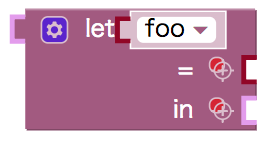
\includegraphics[keepaspectratio, scale=0.3]{img/boundFoo0.png}
 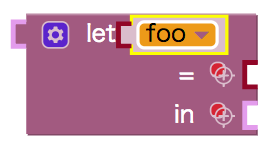
\includegraphics[keepaspectratio, scale=0.3]{img/boundFoo1.png}
 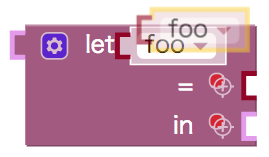
\includegraphics[keepaspectratio, scale=0.3]{img/boundFoo2.png}
 \caption{変数ブロックを生成する流れ.変数宣言を囲うように描画されたブロック(左)にカーソルを合わせて(中)ドラッグする(右)と,
変数ブロックの生成を行うことができる.\label{fig:boundFoo}}

 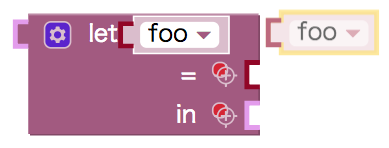
\includegraphics[keepaspectratio, scale=0.3]{img/refBlock0.png}
 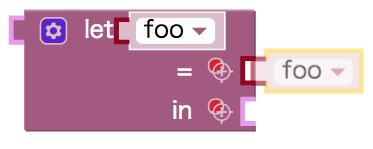
\includegraphics[keepaspectratio, scale=0.3]{img/refBlock1.png}
 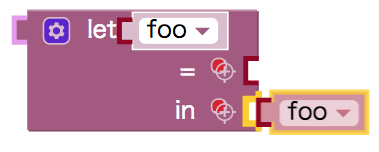
\includegraphics[keepaspectratio, scale=0.3]{img/refBlock2.png}
 \caption{変数ブロック「{\tt foo}」を生成後にドラッグしたまま動かしたときのブロックの様子.
正しく変数ブロックが束縛されない場合はブロックを不透明に表示する.\label{fig:refBlockFoo}}

 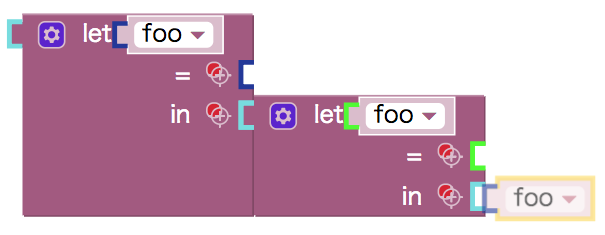
\includegraphics[keepaspectratio, scale=0.3]{img/dupFoo0.png}
 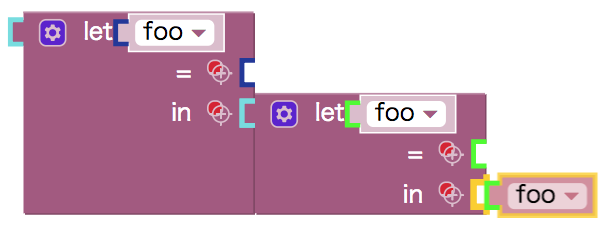
\includegraphics[keepaspectratio, scale=0.3]{img/dupFoo1.png}
 \caption{外側の変数宣言部分から生成した変数ブロック(左)と,
内側から生成した変数ブロック(右)を内側のin以下に接続させようとしたときの比較.
変数ブロックのコネクタの色にも注目されたい.\label{fig:dupFoo}}

 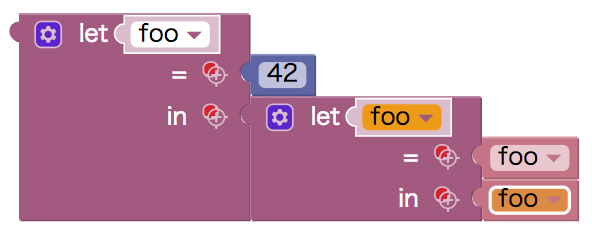
\includegraphics[keepaspectratio, scale=0.3]{img/dupFooInt42.png}
 \caption{右下の変数ブロックをホバーしたときの反応.束縛変数,
束縛されている変数がオレンジ色にハイライトされる.\label{fig:dupFooHover}}
\end{figure}

\section {スコープお砂場}
変数ブロックや変数ブロックを含むブロックをスコープが有効な場所にしか置けないという制約を設けると,
ブロックを自由な場所に置き,好きな順番でブロックを組み立てられるという,本来のBlocklyにあった利点を損なってしまう.
これを避けるため,本研究では,スコープチェックのついた遊び場を設け,これを「スコープお砂場」と命名した.使用例を図\ref{fig:osunaba}に示す.

スコープお砂場は新しい変数が加わりうる各入力コネクタに紐づいており
\footnote{図\ref{fig:osunaba}では,inの直前のスコープにもお砂場のためのアイコンが表示されているが,
これはletに引数を追加する場合やrecフラグを有効にした場合に必要になる.},
コネクタの隣にあるアイコンをクリックするとポップアップの形で表示される.
所属先のコネクタから参照できる変数の一覧がお砂場内のフライアウトメニューから見られるようになっていて,そこから変数ブロックの生成も行える.
ユーザはこのスコープお砂場でブロックを適当に組み合わせたのち,目的のブロックと接続をすればよい.
スコープお砂場は,入れ子にしても使うことができる.

このお砂場にはスコープチェックがついており,
所属先のコネクタから参照することができない変数を含むブロックはお砂場に移動することができない.
例えば図\ref{fig:osunaba}の右下のお砂場にある「{\tt foo}」ブロックはもう一方のお砂場に移動できるが,
「{\tt bar + ?}」のブロックは移動することはできない.ブロックが不透明になり,
ブロックをそのままリリースしてもブロックの移動はキャンセルされる.

また,お砂場を所有するブロックが移動する際は,お砂場内のブロックもスコープチェックの対象である.
例えば,図\ref{fig:osunaba}の「{\tt let bar = ?\ in ?}」を表すブロックを動かして「{\tt let foo = ?\ in ?}」の2つ目のスコープから外した場所に置くことはできない.
お砂場内に変数ブロック「{\tt foo}」が存在しているためである.

% 一番大変だったわりに説明がすくねえ
\begin{figure}[h]
 \centering
 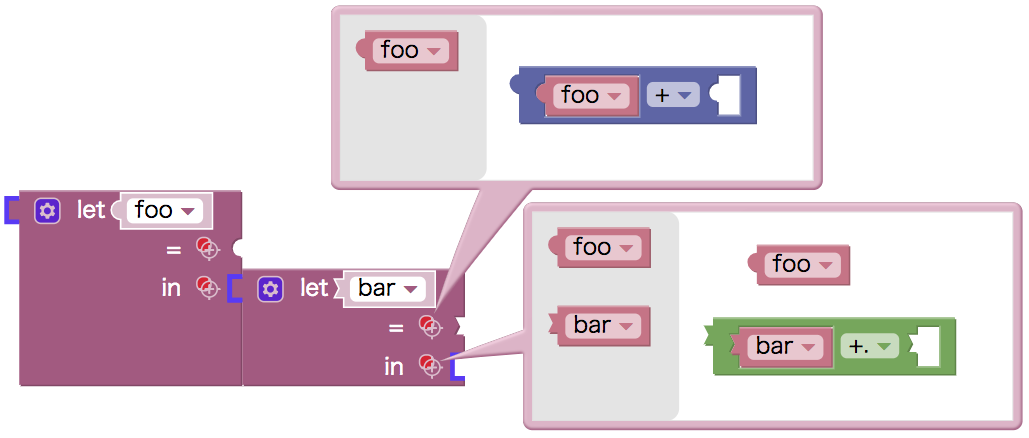
\includegraphics[keepaspectratio, scale=0.3]{img/osunaba3.png}
 \caption{スコープお砂場の例.ライフルのスコープを模したアイコンをクリックするとポップアップが現れる.
スコープで参照できる変数ブロックの一覧が見れ,ブロックの生成も行える.
スコープお砂場内で,変数ブロックをどんな型として扱うかによって,変数宣言のブロックの型も変化する.\label{fig:osunaba}}
\end{figure}

\section {let多相を含んだ型システム}

let多相を含む型システムを実装した.
また,型の単一化の解除をサポートした.
例えば,リストコンストラクタのブロック「{\tt ?\ ::\ ?}」にint型ブロックを入れて「{\tt 3 ::\ ?}」とすると,
出力コネクタの型が{\tt 'a list}から{\tt int list}へと更新されるが,{\tt int}型ブロックを外すと再び{\tt 'a list}型に戻る.

同じ変数の型は,例えば図\ref{fig:osunaba}の変数「{\tt bar}」のように,スコープお砂場に置かれたブロックであっても一貫していなければならないとした.
例えば,スコープお砂場の外で宣言された変数を参照する変数ブロックが,
スコープお砂場内で{\tt float}型として扱われたならば,元の変数宣言も{\tt float}型であると決定される.

\section {メッセージ出力\label{fun:message}}

不正なプログラムを組み立てられないユーザインタフェースを設けると,
なぜ不正なのかをまだ理解できない初学者が困惑してしまう可能性があり,
本研究が達成するべき「理解しやすさ」が不十分になってしまう.
これを回避するため,本システムではドラッグ中のエラーを書いたツールチップの表示を行った(図\ref{fig:errorOutput}).
なぜユーザの意図した場所にブロックを置くことができないのか,
なぜ目的のブロックと接続できないのかといった理由を見ることができる.エラーのフォーマットは,本来のOCamlのエラー出力になるべく従っている.

\begin{figure}[h]
 \centering
 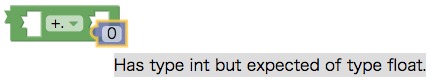
\includegraphics[keepaspectratio, scale=0.4]{img/errorIntFloat.png}
 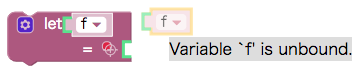
\includegraphics[keepaspectratio, scale=0.4]{img/errorUnbound.png}
  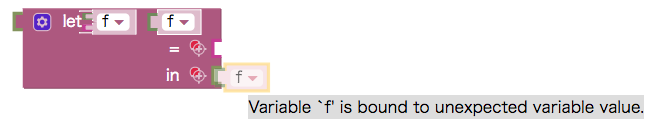
\includegraphics[keepaspectratio, scale=0.4]{img/errorDupVar.png}
 \caption{エラーツールチップの例.\label{fig:errorOutput}}
\end{figure}



\chapter{実装方法}\label{chap:impl}

前章では,OCaml Blocklyが4つの主な機能をユーザから見た視点で紹介した.
本章では,それぞれについて実装方法を詳細に説明する.本研究はBlocklyに加え\cite{Typed-Blockly}もベースにして行っているため,それぞれの実装も交えて説明を行う.

\section {変数束縛\label{impl:boundVariable}}

まず,Blocklyでの変数ブロックの実装について触れる.Blocklyでは,新しい変数の追加をフライアウトメニュー内にあるメニューボタンから行う.既に存在する変数名の追加は行えない.変数を追加すると,図\ref{fig:blocklyVar}のような変数フィールドを持った数種類のブロックがフライアウトメニューに追加される.変数フィールドとは,図\ref{fig:blocklyVar}の変数名iを囲う薄いピンク色の部分であり,クリックすると変数名の変更などが行えるブロック内のエレメントである.
各変数フィールドは,内部的に変数インスタンスを保持している.
例えば,図\ref{fig:blocklyVar}に示した3つの変数フィールドは,1つの変数インスタンスを内部的に共有している.
そうすることで,変数名を変更したときに,同じ変数を参照する変数フィールドの変数名が同期的に更新される.
しかし,このBlocklyでの変数の扱いは,関数型言語でのimmutableな変数やシャドウイングをわかりやすく表現するためには相性が悪い.
Blocklyにはスコープという概念がなく,全ての変数はグローバルな変数として扱われており,同名の複数の変数を扱うことができないためである.

\begin{figure}[h]
 \centering
 
\includegraphics[keepaspectratio, scale=0.3]{img/iVar.png}
 \caption{Blocklyにて,ブロック内に変数フィールドを持つ3つのブロックの例.\label{fig:blocklyVar}}
\end{figure}

束縛変数とその束縛関係を表現するために,変数インスタンスの種類を「宣言される変数」と「宣言される変数を参照する変数」に分ける.参照する変数は,自身がどの変数を参照しているのかを保持し,変数名を取得したいときや変更したいときはそれに問い合わせれば,変数名が変更されたときの各変数フィールドの更新をBlocklyと同様にシンプルに行うことができる.

変数宣言と変数参照という2種類の変数インスタンスを用いて,スコープチェックを以下のように実装した.
変数宣言を持つブロックには,スコープを作るコネクタを引数として,スコープ内で参照できる変数の一覧を返す関数を定義する.
この関数を用いて変数環境を更新して,スコープ内のブロックに存在する全ての変数参照が変数環境にあるかどうかを調べれば良い.
この作業を再帰的に行えば,ネストしたブロック全体のスコープチェックが行える.
ユーザがある 2 つのコネクタを接続しようとしたときは,接続を仮定したスコープチェックを行い,失敗した場合は接続を拒絶する.

次に,拡張された変数フィールドの描画について説明する.
変数宣言か変数参照かどうかによって変数フィールドの描画の仕方を変える.
変数宣言の場合は,ブロックの形を変数フィールドの背景に描画し,変数宣言部分から変数ブロックの生成を行えることを表現する.
そして,実際にドラッグされたときにその変数への参照を持つブロックを生成する.
変数フィールドをホバーしたときに,関連した全ての変数フィールドをハイライトする機能は,変数宣言が自身を参照する変数の一覧を保持することによって行える.
変数宣言に問い合わせて関連した全ての変数を取得したら,それら変数を内包する各フィールドの背景色を変える.

\section {スコープお砂場\label{impl:osunaba}}

スコープお砂場のようなメインワークスペースとは独立した作業空間を実現するには,まずワークスペースをもう1つ作ればよい.
そうすることによって,メインワークスペースとは分離した別のブロックを組み立てる世界を作ることができる.

スコープお砂場内でのスコープチェックはメインワークスペースとは異なる.
メインワークスペースでのスコープは空の変数環境であるが,お砂場でのスコープは所属先のスコープで使える変数を全て含んだ変数環境である.
このお砂場が持つスコープは,お砂場を所有するブロックを上位から辿っていくことにより取得する.
これは,構文木を上から辿って変数環境を更新していくインタプリタと似た要領である.
お砂場が入れ子になっている場合は,親のお砂場が持つスコープも同様に取得する.
ユーザがブロックをお砂場の上にドラッグしてきたときには,移動中のブロック内の自由変数が全てお砂場のスコープで有効かを調べる.
そうでない場合は,お砂場内で参照できない変数を含んでいるときなので,ブロックのお砂場への移動を拒絶する.

また,スコープから参照できる変数ブロックを並べたフライアウトメニューをお砂場に実装した.これによって,ユーザはお砂場内で使用できる変数の一覧を知ることができ,また,変数参照ブロックの生成も直接そこから行うことができる.
スコープお砂場を所有するブロックの移動によって,お砂場の暗黙的な変数環境が変わるときは,即時的にフライアウトメニューを更新する.

お砂場にブロックを持ちよって自由に組み立てたり,その後に別のワークスペース内のブロックと接続させたりするには,ブロックが異なるワークスペース間を移動できるようにする必要がある.
Blocklyでは,ブロックの自由な組み立てはメインワークスペースでしか行われないため,ワークスペースを越えたブロックの移動は想定されていない.
このため,本システムではブロックのワークスペース間の移動を実装した.実装の方法は主に2つあると考えられる.

1つの方法はブロックのSVGを移動先のワークスペースのSVGグループに移動させ,ブロックオブジェクト内の古いワークスペースへの参照を全て更新することである.%先行研究は過去形に????
この方法はあまり現実的でない.
なぜならワークスペースと繋がりを持つのはブロックのみでなく,コネクタやフィールドなどといったブロック上に存在する不特定多数のコンポーネントも,ワークスペースを参照し合ったり,イベントリスナーを登録したりするなどしてワークスペースに依存しているためである.それら全てのワークスペースへの依存を完全に正しく更新するのは煩雑であり,将来の拡張のたびに変更が必要な,技術的負債となりうる.
%BlocklyをベースにすることでUIの実装を省いているため,Blocklyの実装を安全に利用したい.

もう 1 つの方法は移動先に新しいブロックを作り直し,古いブロックを削除することである.
この方法は, Blockly に元々あるブロックのエンコード,デコード機能をうまく使うことによって,比較的容易に確実な実装をすることができる.

\subsection*{XMLを利用したブロックの再構築}

Blockly では,ブロックをXML にエンコード,XMLからブロックにデコードできるようになっている.
このブロックとXMLの双方向の変換は,Blocklyにていろいろな場面で活用されている.
例えば,デモページを作るとき,フライアウトメニューにどの種類のブロックを備えるかはXMLで指定することになっている.
指定するXMLを入れ子にすれば,接続した複数のブロックをフライアウトメニュー上に並べることもできる.
%例えば,フライアウトメニューからブロックを生成する際には,元型のブロックをXMLにし,メインのワークスペースにてXMLに従ってブロックを作り上げることによって行なっている.

本研究では,このブロックとXMLの双方向変換を利用して,ワークスペース移動時のブロックの再構築を行なった.
移動したいブロックを XML にエンコードし,その XML から新しいブロックをデコードして得る.
このとき,ブロック内の変数の参照関係が新しいブロックでも保たれるように注意しなければならない.
移動するブロックの中に自由変数,つまりブロックの外側で宣言された変数を参照する変数がある場合,元の変数への参照を XML にエンコードすることによって,適切に参照を保つように実装した.

なお,XMLをデコードして新しいブロックを組み立て直す最中はブロックに対するスコープチェックを無効にする.
ブロックは深さ優先で組み立てられていくが,例えば「{\tt let x = ... in x + 42}」の足し算ブロック部分「{\tt x + 42}」を組み立てる最中に,{\tt x}がスコープにない変数になってしまうからである.また,ブロックに付属したスコープお砂場も同様に新しいブロックへと移動させるが,その説明はここでは割愛する.
% let f = f + x を let x = d + d in 

\section {let多相を含んだ型システム\label{katasuiron}}

Blocklyは型を文字列による名前で表現することによって,簡単な型チェックをサポートしている.各コネクタに型の名前を保存することができ,型が設定されている場合は,同じ名前の型を持つコネクタとしか接続できないようにすることで,単純な型付けを行なっている.

型を文字列で区別してしまうとList型などのパラメタ付き型を表現することは難しいが,
\cite{Typed-Blockly}では各コネクタに文字列の代わりに型変数などの型表現を加えることによってパラメタ付き型をブロック上に実装している.
型の単一化が可能な型表現を持つコネクタ同士でしか接続できないようにし,接続する際には2つのコネクタが持つ型表現を単一化する.
一方で,\cite{Typed-Blockly}では連結させたブロックを外したとき型の単一化が解除されないことや,構文に沿った型推論,let多相が実装されていないなど,拡張が必要な部分があった.

\subsection*{型の単一化の解除}
ユーザがブロックを外した際に型の単一化の解除を行うには,コネクタに添付した型変数の単一化の関係を全て削除したのち,構文の意味に沿ってもう一度型推論を走らせることが必要である.
新しい型変数を振り直すことも単一化解除の1つの方法だが,本システムでは型変数を固有の色で表現しており,解除後にも同じ色を保つ必要があるため,型変数の振り直しは行わない.
型付きブロックのクラス定義それぞれに,以下の2つインスタンス関数を定義する.
\begin{description}
 \item[{\tt clearTypes()}] ブロックに存在する全ての型変数の単一化の関係を削除する.
 \item[{\tt inferTypes(env)}] ブロックの構文に沿って型推論を行う.
引数{\tt env}は型環境であり,変数名をキーとして型スキームを値として持つオブジェクト.返り値としてブロックの出力の型を返す.
\end{description}

ある2つのブロックの接続が外れたとき,全ブロックのトップのブロックから{\tt clearTypes},{\tt inferTypes}を順に実行すればよい.

\subsection*{let多相の実装} %letたそうの説明加える?
let多相を実装するには,ブロックの接続解除時だけでなく,接続時にもトップのブロックから型推論を実行する必要がある.
値制限を設けているためブロックの付け替えによって単相,多相との切り替えが起こりうるためである.
また,スコープお砂場にあるブロックにも型推論を行うことを考えると,型推論を行うブロックの順番も重要である.
束縛型変数を持つ型スキームの場合,letで宣言した変数の型スキームの解決は,必ずスコープお砂場にあるブロックに型推論を走らせるよりも前に行わなくてはならない.スコープお砂場にletで宣言した変数に束縛された変数ブロックに対して型推論を行うとき,その型スキームが必要になるからである.
% https://developers.google.com/blockly/guides/create-custom-blocks/type-checks

\section {メッセージ出力}

第\ref{chap:features}章で述べた通り,本研究で防ぐ対象とするエラーは,シンタックスエラー,型エラー,Unbound valueエラーの3つである.
シンタックスエラーはブロック上では起き得ないとして,ドラック中のメッセージ出力は型エラー,Unbound valueエラーの2つに対して行うとする.

ユーザになぜ期待通りの動作が行えないのかを説明するべきシーンは,以下の2つがある.
\begin {itemize}
  \item 接続してしまうと型エラーあるいはUnbound valueエラーが起きてしまうコネクタ同士を繋げようとしたとき.
  \item 変数を含んだブロックを変数環境に正しく束縛されず,Unbound valueエラーが起きてしまう場所にドラッグしたとき.例えば,「{\tt x; let x = 5}」など.
\end {itemize}

1つ目におけるエラーを取得するためには,接続可能なコネクタを探索する処理を拡張する.
Blocklyには,近傍にあるコネクタの中から接続可能なものを探す処理がある.
この接続可能かどうかの判断はOCaml Blocklyのために拡張されたため,第\ref{impl:boundVariable}節で触れたようなスコープチェックや,型チェックが含まれている.
近くのコネクタが全て接続可能でない場合,最も近いコネクタに対するエラーメッセージをツールチップに表示する.
このエラーメッセージは,Unbound valueエラー,型エラーに関する詳細をユーザに通知する.

2つ目は,ブロックを接続させずに移動させる動作になる,すなわち,十分に近いコネクタが存在しない場合である.この場合は,ドラックされているブロックに対してスコープチェックを行い,正しく変数環境に束縛されない変数が存在するならば,そのエラーメッセージを取得し,表示すればよい.




\chapter[ブロックとOCamlコードとの相互変換]{ブロックとOCamlコードとの\\相互変換}\label{chap:converter}


本節では,ブラウザ上でのブロックとOCamlコードの相互変換の実現について説明する.
組み立てられたブロックからOCamlコードを生成することで,
本来のテキストによるOCamlプログラミングへのイメージが湧きやすくなる.
逆にOCamlコードからブロックへの変換を実現することで,
型や変数の束縛関係を視覚的に確認できることになり,
テキストベースのプログラミングに移行しつつある初学者にとっての補助となることが期待できる.
また, OCaml コードから複雑なブロックの組み合わせを復元できるので,
OCaml Blocklyの開発時に,
特定の条件下のUI/UXをテストしたいときに使うこともできる.
双方向の変換について,それぞれ説明を行う.

\section {ブロックからOCamlコードへ}
第\ref{chap:intro}章で述べた通り,
Blocklyは標準のブロックに対してJavaScriptやPythonなどのスクリプト言語へのコード生成をサポートしている.
それらの実装と同じような手順で,
本研究で新たに追加したOCamlブロックに対するOCamlコードの生成を実装した.
ブロックは構文木と一対一対応しているので,
OCamlコードへの変換は比較的自明である.
% デザインレシピをともに出力する。
\section {OCamlコードからブロックへ}
%まだ実験的な実装だけど.
第\ref{impl:osunaba}節で述べた通り,BlocklyはブロックとXMLのエンコード,
デコードをサポートしている.
つまり,OCamlコードをブロック表現のXMLに変換することができれば,
ブロックを生成することができる.
OCamlコードをパーズするために,
OCamlコンパイラのパッケージcompiler-libsを利用した.
入力されたOCamlコードからcompiler-libs によって抽象構文木を得たのちは,
木をトラバースして対応するブロックの XMLを組み立てる.
これらをビルドしたものをjs\_of\_ocamlでJavaScriptへと変換すれば,
ブラウザ上でOCamlコードからブロックへの変換が実現できる.
変換するコードの例を図\ref{OCamlWallis}に,
コードをブロックに変換したものを図\ref{fig:piOCaml}に示す.

\begin{figure}[h]
\centering
\begin{verbatimtab}[2]
let rec pi_impl n d =
  if n > 0.0
  then n *. n /. d /. (d -. 2.0) *. pi_impl (n -. 2.0) (d -. 2.0)
  else 1.0;;
let pi n = 2.0 *. pi_impl (n *. 2.0) (n *. 2.0 +. 1.0);;
let pi_exp = pi 9000.
\end{verbatimtab}
\caption{ウォリス積を利用して円周率を計算する OCaml プログラム\label{OCamlWallis}}

 \centering
 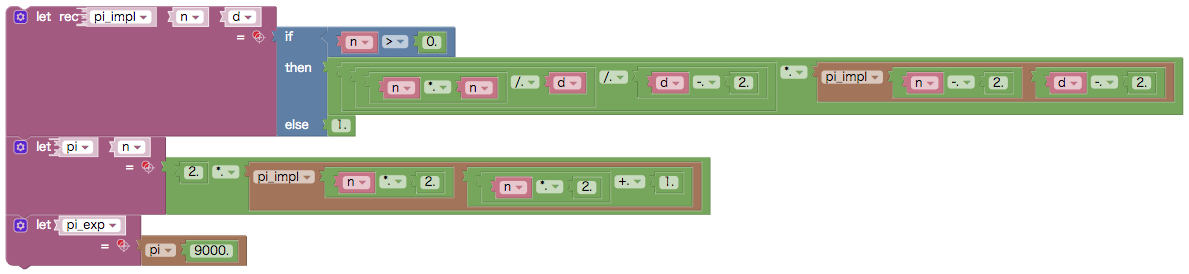
\includegraphics[keepaspectratio, scale=0.35]{img/pi.png}
 \caption{図\ref{OCamlWallis}に現したウォリス積を利用したOCamlプログラムをブロックに自動で変換したもの.
型の整合性,変数束縛ともに反映されている.\label{fig:piOCaml}}
\end{figure}


\chapter {現状と実使用に向けて}\label{chap:todo}

\section {現状}\label{sub:genjo}

シンタックスエラー,型エラー,Unbound valueエラーが起きないという制約の元に,OCamlに慣れるために必要な基礎的な構文を備えた.
現在OCaml Blocklyでサポートしている型や構文は,以下の通りである.使用例を図\ref{fig:ocamlBlocks}に示す.
\begin{itemize}
  \item {\tt bool}型,{\tt int}型,{\tt float}型,{\tt string}型.
  \item 2つ組のみのタプル,リスト,ラムダ式,関数適用.
  \item 論理演算,数値演算,{\tt fst},{\tt snd}などのビルトイン関数.
  \item リストのパターンマッチを行う{\tt match}文.
  \item {\tt in}を持つ{\tt let},{\tt in}を持たない{\tt let},{\tt let rec}(どの{\tt let}もコンテキストメニューから変更可.).
  \item 高々2引数を持つコンストラクタ定義.
\end{itemize}

\begin{figure}[h]
 \centering
 \includegraphics[keepaspectratio, scale=0.35]{img/ocamlBlocks3.png}
 \caption{OCaml Blockly でブロックを組み立てた例.整数を受け取りその階乗を返す関数fac (上)と,整数の入ったリストを受け取りその合計を返す関数sum (中),関数を受け取りそれを実数 7 に二回適用する関数 twice7 およびその使用例 (下).\label{fig:ocamlBlocks}}
\end{figure}

\section {実使用に向けて}\label{sub:later}

第\ref{chap:senko}章にて掲げた最終的な目標は以下の2つであった.
\begin {enumerate}
  \item コンパイルエラーを起こすプログラムは組み立てられないようにする.
  \item 関数型言語初学者向けの授業で使えるクオリティにする.
\end {enumerate}

本論文では,この最終的な目標を見据えた上で,そのproof of conceptとなる目標を達成することができたと考えている.
今後は,現状のOCaml Blocklyの元にさらなる実装やテストを重ね,最終的な目標を達成していきたい.
そのために具体的に何を行なっていくか,どんな困難があるのか,といった点を本章で整理し,考察する.

\subsection*{コンパイルエラーの起きない制約}

本論文では,シンタックスエラー,型エラー,Unbound valueエラーを主要なコンパイルエラーとし,
この3つのエラーを起こすプログラムの組み立てを制限したユーザインタフェースを実装した.
%ブロックに穴があれば,生成されたプログラムは余裕でシンタックスエラーになってしまうため,ユーザへの警告が必要.
Unboundに関するエラーとしては,以降レコード型などの構文を追加していくに当たって,Unbound fieldなどといったエラーが起きうることが考えられるが,これはUnbound valueエラーを防いだ実装と同じような要領で回避することができる.

一方で,標準のOCamlで起きうるコンパイルエラーはシンタックスエラー,型エラー,Unboundエラーの3つだけではない.
例えば,「{\tt let rec f = f}」というプログラムは,2つ目の{\tt f}の出現を指して,「{\tt This kind of expression is not allowed as right-hand side of `let rec'}」というコンパイルエラーになるし,「{\tt match ... with x ::\ x -> ...}」といったプログラムは
2つ目のパターン変数{\tt x}を指して「{\tt Variable x is bound several times in this matching}」というエラーになってコンパイルが失敗する.

これらのコンパイルエラーを起こすプログラムをブロック上で組み立てられないよう,
OCaml Blockly上でのエラーのチェックを拡張していく必要があるが,その方法は主に2つある.

1つは,各種エラーを逐一対応していき,アドホックな変更を重ねることである.
この方法は,数種類のエラーだけを対応するならば,手っ取り早く確実であるが,
全てのコンパイルエラーを防ぐためには,スケールしない方法と言える.
OCaml BlocklyはOCamlという膨大な言語処理のとても局所的な部分をJavaScript上で「再現」しているため,
OCamlにおけるコンパイルエラーと一貫性を保つのは困難である.

2つ目の方法は,compiler-libsを利用して実際にコンパイルを行い,そのコンパイルエラーを流用することである.
抽象構文木にブロック上の穴を表現するための構文を追加し,ブロックを抽象構文木に落せるようにして,コンパイルを行う.
コンパイルエラーが起きたら,そのエラーを返す.このプログラムをビルドしたものをjs\_of\_ocamlでJavaScriptに変換し,ブラウザ上で用いる.
この方法は,OCamlにおけるコンパイルエラーとの一貫性を確実に実現できるが,
お砂場を含むワークスペースにある全ブロックとテキストによるOCamlコードの対応関係を的確に保たなければいけない.

\subsection*{さらなる構文}

新しい構文をただ単にブロックに追加するのは容易であるが,
「不正なプログラムを組み立てられない」というOCaml Blocklyの制約を維持しながらの構文の追加は自明でない.

例えば,ユーザの動作によってあらゆる箇所のブロックが動的に変更された場合にどう対応するかという仕様を考えなければならない.
コンストラクタを定義するブロックが変更されたとき,コンストラクタ呼び出しはどう変わるべきか,その引数に自由変数が入っていたらどうなるべきか,などを検討しなくてはならない. % といった問題がある??

他にも,ブロックのユーザインタフェースとどう合わせるのかを考える必要がある.
例えば,変数を持つパターンブロックがmatchブロックに接続されたときに,変数宣言としてどう見せるべきなのか,
可変長の要素を持つブロックであれば,それをどうユーザに操作させるのが適切か,などといった問題がある.
これらの問題を考えると,構文と構文が表す概念をOCaml Blocklyの世界に載せるには時間が必要である.

本論文では,ユニットテストで様々な組み合わせのプログラムを機能させ続けることに注意を払つつ,
OCaml Blocklyでの各構文の仕様を決め,種類を少しずつ足していった.
基礎的な構文が実現できた今,OCamlの授業で使用するために,次に追加する必要のある構文を以下にまとめた.

\begin{itemize}
  \item 柔軟なコンストラクタ定義,レコード型.
  \item 可変長のタプル.
  \item 豊富なマッチパターン.
\end{itemize}

OCamlで様々なデータセットを扱うために,コンストラクタ,レコード型といった柔軟なユーザ定義のデータ型を実現したい.
また,現状ではタプルは2つ組のみしかサポートしていないが,可変長のタプルを追加する.
次は,関数型言語の重要な特徴の1つといえるmatch文のパターンを豊富にすることである.
現在は{\tt x ::\ xs},{\tt []}といった2つのパターンのみが使えるが,これを拡張し,
例えば{\tt (a, b)}や,再帰的なパターン{\tt (a, b) ::\ xs}を表現できるようにする.

これ以上の構文は,実際に授業のカリキュラムに合わせてテストをした際に,
必要な構文があれば随時サポートしていく指針である.
%もっと最終目標言うべき?

\subsection*{ユーザビリティの点から}

使いやすさ,理解しやすさを達成するためには,まず第一に初学者にテストしてもらいフィードバックをもらう必要がある.
フィードバックに基づき,OCaml Blocklyのユーザインタフェースに関わる部分を改善していく.

一方で,著者が実際に使用してみたとき,実使用に向けて,使い勝手の点から設計や実装が必要だと考える点は以下の2つである.%4つ?
\begin{itemize}
 \item 構文の意味に沿ったブロックのデザインの改造.
 \item 型を視覚的に表示することの限界.
% \item Undo機能の実装.
\end{itemize}

まず始めに,OCamlの構文が持つ意味に合わせて,ブロックのデザインを改造する必要がある.
現在ブロックそのものの見た目はほとんど変えていない.
もともとBlocklyはビジュアルプログラミング言語環境を構築するためのライブラリであり,
1つの言語に特化した設計にはなっていないが,
どちらかというと命令型言語との方が相性が良く,関数型言語のような文より式が主な言語をそのまま載せると,
Blocklyにあった直感的なユーザ体験を損ないがちである.図\ref{fig:ocamlBlocks}では,letブロックの左側の余白部分が大きいせいで,代入や出力の関係が捉えにくくなってしまっている.
初学者にとってOCamlの言語仕様をより直感的に理解してもうらためには,
OCamlの言語仕様に特化したビジュアルのデザインが不可欠である.

また,型を視覚的に表示することには限界がある.
型によってコネクタの形を変える\cite{Typed-Blockly}のアイデアは,
プリミティブ型に関してはとても有効である.
一方で,Function型などといったパラメタ付型を形で表すと,型が入れ子になって複雑になるほど,視認性が低くなってしまう.
このことが特に問題となりやすいのは,高階関数を使用する際である.
OCaml Blockly では高階関数を扱うことができ,例えば,関数を受け取りそれを実数7に二度適用する関数 twice7 (図\ref{fig:ocamlBlocks})や,関数 map,fold などのプログラムを組むことができる.
しかし,高階関数は型が深い入れ子になりやすいため,そのまま描画してしまうと型を視認しづらくなってしまい,初学者を困惑させうる.
これを防ぐため,現段階では,Function型を持つ変数ブロックを高階関数としてではなく,引数の数だけ穴を持った関数適用として生成している.
高階関数のように深い入れ子になっている型を初学者にわかりやすく見せるためには,そのような型の情報を視覚的に描画する代わりに,ホバー時にツールチップの形で出力する,などといった新しい策を考える必要がある.

%最後の1つは,OCaml Blocklyでのundoの実装である.%この段落の説明が微妙
%ユーザが誤ってブロックを削除してしまったとき,undo機能があればストレスなく元の作業に戻ることができる.
%blocklyではundoやredoが実装されているが,
%作業空間がメインワークスペースのみであるために,undo機能を実現するためのユーザの動作の記録はメインワークスペースのみに行われている.
%対して,OCaml Blocklyにはお砂場という別の作業空間があるため,動作の保持をグローバルに行うよう拡張する必要がある.

%是非そういうところに注目してみてほしい!!

% blockly/blockly/demos/interpreter/step-execution.html




\chapter {結論}\label{chap:conclusion}

ビジュアルプログラミング環境構築のためのライブラリBlocklyをベースにして,
OCamlプログラムを組み立てるビジュアルプログラミング環境,OCaml Blocklyを開発した.
束縛変数,let多相を含む型システムを実装し,シンタックスエラー,型エラー,Unbound valueエラーを起こすプログラムの組み立てを拒否するユーザインタフェースを構築した.
変数ブロックを用いた自由なブロックの組み立てを行うことができる,スコープチェックの付いた空間,スコープお砂場を実装した.
ユーザが理解しやすいエラー出力や,
OCaml言語に慣れるために必要な基礎的な構文のサポート,
テキストベースのプログラミングへの導入となるブロックとテキストとの相互変換を行った.

実使用に向けた課題は第\ref{sec:seiri}節にてまとめたが,それとは独立して,OCaml Blocklyには更に高度な拡張に向けた展望がある.
例えば,Try OCamlを用いてブラウザ上でのOCamlコードの実行をサポートすることが考えられる.
他にも,本学の授業で既に用いられているデバッグツールである,型デバッガ\cite{10.1007/978-3-642-41582-1_12}との融合も考えられる.
型の整合性を壊すようなコネクタを接続させようとしたときに,ブラウザ上に型デバッガを起動させれば良い.
そうすれば,本論文が第\ref{fun:message}節で行なった,2つの型がなぜ合わないかのエラー出力だけでなく,ユーザの意図したプログラムの型が破綻した原因は
どの箇所にあったのか,という型の間違いを発見することができる.

これからOCaml Blocklyを実使用していくことに向けて,本システムをさらに拡張,改善していきたい.
OCaml Blocklyの実装は,https://github.com/harukamm/ocaml-blocklyにて公開されている.



\newpage
\chapter*{謝辞}

大変丁寧にご指導してくださり,貴重なご意見をたくさんくださった浅井先生に感謝します.
実用的なご意見やご指摘をくださり,PRを出すなどして親身になって協力してくださった研究室の方々には,大変励まされました.感謝します.
友人として近況を報告し合い,励まし合ったS線香花火氏,中川氏に感謝します.
%他愛のないどうしようもない話ばかりし合い,いつでも中学時代のような気持ちに戻らせてくれた古藤氏に感謝します.
貴重な体験をさせてくれた両親に感謝します.
修士学生の間に技術的な数々のことを教えて頂き,
相談に乗ってくださったプログラマS氏に感謝します.


\newpage
%参考文献をしめします.


\begin{thebibliography}{3}
\bibitem {bunken} 参考文献は,本または論文のタイトル,著者名,出版社,ページ(論文の場合),発行年を記すこと.
\bibitem{latex2e}
乙部巌己,江口庄英,
pLaTeX2ε for Windos,SOFT BANK,1996.
\end{thebibliography}


\newpage

%付録
%\appendix
%\chapter{実験でもちいたデータ}

ここには,実験のデータなど,論文の本文中に載せられなかったが,
読者にとって役に立つとおもわれるデータなどを付録として掲載する.

\chapter{ふろく}

\section{section}

\section{2}

\chapter{furoku}


\end{document}
